% !TeX root = ../complete.tex
\section{تخمین \lr{Activity Factor}}
\label{sec:power-activity}

\subsection{شمارش از روی دنباله نمونه‌ها}
\label{sec:power-activity-trace}

اگر شکل موج واقعی در دسترس باشد، می‌توان لبه‌های صعودی را در بازه‌ی
مشاهده شمرد و از رابطه \eqref{eq:power-activity-count} استفاده کرد.
اگر فقط یک نمونه از مقدار منطقی در هر مرز دوره داشته باشیم، شمارش
از روی نمونه‌ها به این فرض وابسته است که بین دو نمونه حداکثر یک
گذار رخ داده باشد. فرض کنید نمونه‌های متوالی یک گره چنین‌اند.
\[
  0\ \longrightarrow\ 1\ \longrightarrow\ 1\ \longrightarrow\ 0\
  \longrightarrow\ 0\ \longrightarrow\ 1\ \longrightarrow\ 0 .
\]
هفت نمونه، شش فاصله‌ی زمانی به طول یک دوره ساعت می‌سازند. فقط
فاصله‌ی اول و پنجم گذار صعودی دارند. پس تخمین \(\alpha\) در این
بازه \(2/6=1/3\) است. سه نمونه مقدار یک دارند، ولی برای توان،
تعداد نمونه‌های یک را نمی‌شماریم. هر بار ورود به سطح یک، متناظر با
شارژ خازن است. نمونه‌ی دوم و سوم هر دو یک‌اند و میان آن‌ها در این
مدل شارژ جدیدی رخ نمی‌دهد.

\subsection{احتمال سطح منطقی و احتمال گذار}
\label{sec:power-switching-probability}

وقتی شکل موج در دسترس نیست، می‌توان فعالیت را از یک مدل آماری
تخمین زد. مقدار منطقی گره در چرخه شماره \(k\) را \(X_k\) بنامید.
\(p_X=\Pr(X_k=1)\) احتمال مشاهده مقدار یک است. فرض می‌کنیم توزیع
در چرخه‌های مورد بررسی ثابت است. چون صفر و یک تنها دو نتیجه‌اند و
احتمال‌هایشان باید به یک جمع شود، \(\Pr(X_k=0)=1-p_X\) است.
برای شارژ، لازم است مقدار ابتدا صفر و سپس یک باشد. احتمال این
رویداد مشترک برابر است با احتمال صفر بودن در چرخه اول ضرب‌در
احتمال یک شدن در چرخه بعد، به شرط آنکه چرخه اول صفر بوده باشد.
اگر در هر فاصله حداکثر یک گذار رخ دهد، داریم
\cite[بخش \secnum{۵.۲.۱.۲}، صفحه ۱۸۷]{weste}
\cite[اسلایدهای ۱۴ و ۱۵]{powerslides}.
\begin{equation}
  \begin{aligned}
    \alpha_X
      &=\Pr(X_k=0,\ X_{k+1}=1)\\
      &=\Pr(X_k=0)\,\Pr(X_{k+1}=1\mid X_k=0).
  \end{aligned}
  \label{eq:power-activity-conditional}
\end{equation}
علامت \(\mid\) به معنی «به شرط» است. اگر مقدار چرخه بعد از مقدار
چرخه فعلی مستقل باشد، دانستن \(X_k=0\) احتمال یک بودن چرخه بعد را
تغییر نمی‌دهد. با این فرض، رابطه‌ی فوق به رابطه زیر تبدیل می‌شود.
\begin{equation}
  \alpha_X=(1-p_X)p_X.
  \label{eq:power-activity-independent}
\end{equation}
مثلاً برای داده مستقل با صفر و یکِ هم‌احتمال، احتمال هر یک از زوج‌های
\((0,0)\)، \((0,1)\)، \((1,0)\) و \((1,1)\) برابر \(1/4\)
است. فقط زوج دوم شارژ ایجاد می‌کند. پس \(\alpha_X=1/4\) است.
برای الگوی پی‌درپی صفر و یک نیز اگر نمونه را با احتمال یکسان از دو
جای ممکن الگو بگیریم، احتمال دیدن یک \(1/2\) است. بااین‌حال، بعد
از هر صفر، یک با قطعیت می‌آید. از رابطه
\eqref{eq:power-activity-conditional} در این حالت
\(\alpha_X=(1/2)\times1=1/2\) می‌شود. بدین ترتیب، احتمال یک بودن
به‌تنهایی برای تعیین فعالیت کافی نیست.

\subsection{از جدول صحت گیت تا فعالیت خروجی}
\label{sec:power-gate-activity}

یک گیت \lr{AND} دوورودی را در نظر بگیرید. از جدول صحت فصل صفر
می‌دانیم خروجی \(Y\) تنها وقتی یک است که هر دو ورودی \(A\) و
\(B\) یک باشند. اگر ورودی‌ها در یک چرخه از هم مستقل باشند و
احتمال یک بودن هر ورودی \(1/2\) باشد، می‌توان احتمال حالت مشترک
را با ضرب احتمال‌ها به دست آورد. علاوه‌براین، اگر زوج ورودی در
چرخه‌های متوالی مستقل باشد، خروجی هم در چرخه‌های متوالی مستقل است
و رابطه \eqref{eq:power-activity-independent} برای آن برقرار است.
پس محاسبه دو گام دارد
\cite[جدول \secnum{۵.۱} و مثال ۵.۲، صفحه ۱۸۷]{weste}.
\[
  p_Y=\Pr(A=1,\ B=1)=\frac12\times\frac12=\frac14,
  \qquad
  \alpha_Y=\left(1-\frac14\right)\frac14=\frac{3}{16}.
\]
استقلال ورودی‌ها در یک چرخه برای محاسبه \(p_Y\) به کار رفت.
استقلال بین چرخه‌ها برای محاسبه \(\alpha_Y\) لازم بود. اگر هر دو
ورودی را به یک سیگنال مشترک وصل کنیم، \(Y=A\) می‌شود و محاسبه
\(p_Y\) با ضرب احتمال ورودی‌ها دیگر معتبر نیست. در مقابل، حتی دو
ورودی مستقل در هر چرخه می‌توانند در طول زمان ثابت بمانند. در آن
حالت ممکن است خروجی یک باشد و درعین‌حال هیچ گذار صعودی رخ ندهد.

اگر دو ورودی با تأخیرهای متفاوت به یک گیت برسند، خروجی می‌تواند
بین حالت‌های ابتدا و انتها پالس کوتاه ناخواسته داشته باشد. برای
نمونه، در \lr{AND}، تغییر ورودی‌ها از \((0,1)\) به \((1,0)\)
ابتدا و انتهای خروجی را صفر نگه می‌دارد. اگر \(A\) زودتر بالا
برود، ورودی‌ها موقتاً \((1,1)\) می‌شوند. اگر این وضعیت به‌اندازه‌ی
کافی بماند، خروجی یک پالس ایجاد می‌کند. این \lr{Glitch} در دو
نمونه‌ی ابتدا و انتها دیده نمی‌شود. برای پالس با دامنه کامل، یک
شارژ اضافی به شمار گذارها اضافه می‌شود. برای پالس با دامنه کمتر،
انرژی را باید از روی شکل موج برآورد کرد. به این ترتیب، در حضور
چند گذار در یک دوره، شمار میانگین گذارهای صعودی حتی می‌تواند از
یک بیشتر شود و مدل تک‌نمونه‌ای برای برآورد توان کافی نیست
\cite[بخش \secnum{۵.۲.۱.۳}، صفحه ۱۸۸]{weste}.

\subsection{مثال اسلاید ۱۶، فعالیت گره‌های \lr{AND} چهارورودی}
\label{sec:power-slide-and-activity}

شکل \ref{fig:power-slide-and-activity} مدار دو‌مرحله‌ای اسلاید
را نشان می‌دهد. فعالیت را از ورودی‌های \(A,B,C,D\) تا گره‌های
میانی و خروجی \(Y\) حساب می‌کنیم.

\begin{figure}[htbp]
  \centering
  \begin{latin}
  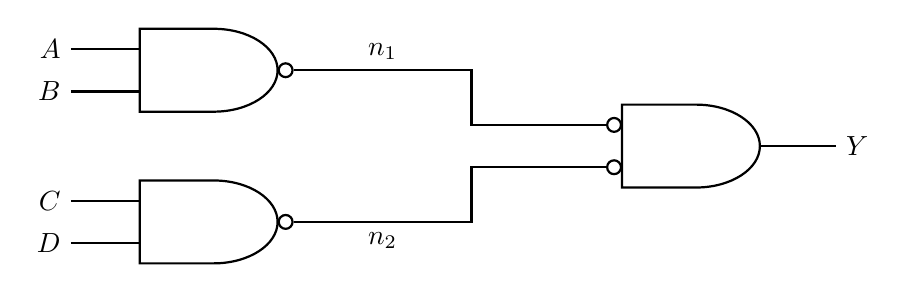
\begin{tikzpicture}[x=1.25cm,y=1.12cm,thick,
      inversion/.style={draw,circle,inner sep=0pt,minimum size=5pt}]
    \foreach \level/\first/\second/\branch in {0.86/A/B/upper,-0.86/C/D/lower} {
      \draw (1.18,{\level-0.47}) -- (1.18,{\level+0.47})
        -- (1.93,{\level+0.47})
        arc[start angle=90,end angle=-90,x radius=0.65,y radius=0.47]
        -- cycle;
      \draw (0.48,{\level+0.24}) node[left] {\(\first\)} -- (1.18,{\level+0.24})
        (0.48,{\level-0.24}) node[left] {\(\second\)} -- (1.18,{\level-0.24});
      \node[inversion,anchor=west] (\branch) at (2.58,\level) {};
    }
    \draw (6.08,-0.47) -- (6.08,0.47) -- (6.83,0.47)
      arc[start angle=90,end angle=-90,x radius=0.65,y radius=0.47]
      -- cycle;
    \node[inversion,anchor=east] (invertUpper) at (6.08,0.24) {};
    \node[inversion,anchor=east] (invertLower) at (6.08,-0.24) {};
    \draw (upper.east) -- (4.55,0.86) node[midway,above] {\(n_1\)}
      |- (invertUpper.west);
    \draw (lower.east) -- (4.55,-0.86) node[midway,below] {\(n_2\)}
      |- (invertLower.west);
    \draw (7.48,0) -- (8.25,0) node[right] {\(Y\)};
  \end{tikzpicture}
  \end{latin}
  \caption{مدار مثال اسلاید ۱۶ با گره‌های میانی \(n_1\) و \(n_2\).
    حباب روی هر پایه مقدار منطقی آن پایه را وارونه می‌کند.
    بازترسیم از اسلاید ۱۶ \cite{powerslides}.}
  \label{fig:power-slide-and-activity}
\end{figure}

دو گیت سمت چپ در خروجی حباب دارند، پس \lr{NAND} هستند.
گیت سمت راست به‌دلیل حباب‌های ورودی، ابتدا هر دو ورودی را
وارونه می‌کند و سپس \lr{AND} می‌گیرد. بنابراین \(Y\) تنها
هنگامی یک می‌شود که \(n_1\) و \(n_2\) هر دو صفر باشند.
این وضعیت دقیقاً زمانی رخ می‌دهد که هر چهار ورودی اولیه یک باشند
\cite[مثال ۵.۲ و شکل \secnum{۵.۹}، صفحات ۱۸۷ و ۱۸۸]{weste}.

فرض می‌کنیم چهار ورودی در هر دوره مستقل و هم‌احتمال‌اند،
بردار ورودی بین دوره‌های متوالی مستقل است و گره‌ها میان
نمونه‌ها گذار اضافی ندارند. پس برای هر ورودی \(p=1/2\)
و \(\alpha=(1/2)(1/2)=1/4\) است. گره \(n_1\) فقط با یک بودن
هم‌زمان \(A\) و \(B\) صفر می‌شود. احتمال آن حالت
\((1/2)(1/2)=1/4\) است. برای \(n_2\)، زوج \(C,D\) همین نقش را
دارد. پس احتمال یک بودن و فعالیت هر گره میانی چنین است.
\[
  p_{n_1}=p_{n_2}=1-\frac14=\frac34,\qquad
  \alpha_{n_1}=\alpha_{n_2}=\frac14\times\frac34=\frac{3}{16}.
\]
دو گره میانی از دو زوج مستقل ورودی ساخته شده‌اند. بنابراین برای
احتمال صفر بودن هم‌زمان آن‌ها، دو احتمال \(1/4\) را در هم ضرب
می‌کنیم. نتیجه با شمارش چهار ورودی هم به دست می‌آید. تنها ترکیب
\((1,1,1,1)\) از میان ۱۶ ترکیب هم‌احتمال، \(Y=1\) می‌دهد.
با اعمال رابطه \eqref{eq:power-activity-independent} بر خروجی داریم.
\[
  p_Y=\frac14\times\frac14=\frac{1}{16},\qquad
  \alpha_Y=\frac{15}{16}\times\frac{1}{16}=\frac{15}{256}.
\]
اگر گره \(n_1\) را وارونه کنیم، احتمال یک بودن از \(3/4\) به
\(1/4\) می‌رسد. در محاسبه فعالیت فقط جای دو عامل
\(p\) و \(1-p\) عوض می‌شود و حاصل همان \(3/16\) است.
